% !TeX program = pdflatex
% !BIB program = biber

\documentclass[
  a4paper,
  11pt,
  ngerman,
  parskip=half,
  bibliography=totoc,
  listof=totoc
]{scrreprt}

% ============================================================================
% PACKAGES
% ============================================================================

\usepackage[left=3cm,right=2.5cm,top=2.5cm,bottom=2.5cm]{geometry}
\usepackage[ngerman]{babel}
\usepackage{csquotes}
\usepackage{xcolor}
\usepackage{acronym}
\usepackage{amsmath, amssymb}
\usepackage{graphicx}
\graphicspath{{img/}}
\usepackage{booktabs}
\usepackage{hyperref}
\usepackage{float}
\usepackage{enumitem}

% ============================================================================
% HYPERREF KONFIGURATION
% ============================================================================

\hypersetup{
    colorlinks=true,
    linkcolor=black,
    citecolor=black,
    filecolor=blue,
    urlcolor=blue,
    bookmarksnumbered=true
}

% ============================================================================
% TITLE PAGE INFORMATION
% ============================================================================

\title{Fragments of Silvaris: Spielanleitung}
\subtitle{Ein 2D Action-RPG}
\author{Aaron Seitz (3006614) \and Robin Fitzek (3006199) \and Burak Yigit (3005865) \and Paul Weber (88487)}
\date{Februar 2026}

% ============================================================================
% DOCUMENT START
% ============================================================================

\begin{document}

% ============================================================================
% TITELSEITE
% ============================================================================

\newgeometry{left=2.5cm,right=2.5cm,top=2.5cm,bottom=2.5cm}

\begin{titlepage}
    \centering

    % HTW Logo
    
\includegraphics[width=0.3\textwidth]{htw.eps}\\[1cm]

    \vspace*{\fill}

    \textbf{\Large Hochschule Aalen}\\
    \textbf{\Large Technik und Wirtschaft}\\[2cm]

    \textbf{\huge Fragments of Silvaris}\\[0.5cm]
    \Large Ein 2D Action-RPG\\[2cm]

    \textbf{\large Spielanleitung}\\
    Spieleprogrammierung --- Wintersemester 2025/2026

    \vspace{3cm}

    \large entwickelt von

    Aaron Seitz (3006614)

    Robin Fitzek (3006199)

    Burak Yigit (3005865)

    Paul Weber (88487)

    \vspace{3cm}

    \large Februar 2026\\

    \vspace*{\fill}
\end{titlepage}

\restoregeometry

% ============================================================================
% INHALTSVERZEICHNIS
% ============================================================================

\tableofcontents

\newpage

% ============================================================================
% ABBILDUNGSVERZEICHNIS
% ============================================================================

\listoffigures

% ============================================================================
% ABKÜRZUNGSVERZEICHNIS
% ============================================================================

\chapter*{Abkürzungsverzeichnis}
\addcontentsline{toc}{chapter}{Abkürzungsverzeichnis}

\begin{acronym}
\acro{RPG}{Rollenspiel (Role-Playing Game)}
\acro{NPC}{Nicht-Spieler Charakter (Non-Player Character)}
\acro{UI}{Benutzeroberfläche (User Interface)}
\acro{XP}{Erfahrungspunkte (Experience Points)}
\acro{HP}{Gesundheitspunkte (Health Points)}
\acro{MP}{Manapunkte (Mana Points)}
\acro{FPS}{Frames Per Second (Bilder pro Sekunde)}
\end{acronym}

\newpage

% ============================================================================
% HAUPTTEIL - SEITENZAHLEN VON ARABISCH
% ============================================================================

\pagenumbering{arabic}
\setcounter{page}{1}

% ============================================================================
% KAPITEL 1: WILLKOMMEN
% ============================================================================

\chapter{Willkommen bei Fragments of Silvaris}

\section{Über das Spiel}

Fragments of Silvaris ist ein 2D Action-\ac{RPG} mit Top-Down-Perspektive, das klassische RPG-Mechaniken mit modernem Spieldesign kombiniert. In einer Fantasy-Welt, die von mysteriösen Slime-Kreaturen bedroht wird, übernimmst du die Rolle eines Helden, der diese Invasion stoppen muss.

\begin{figure}[H]
    \centering
    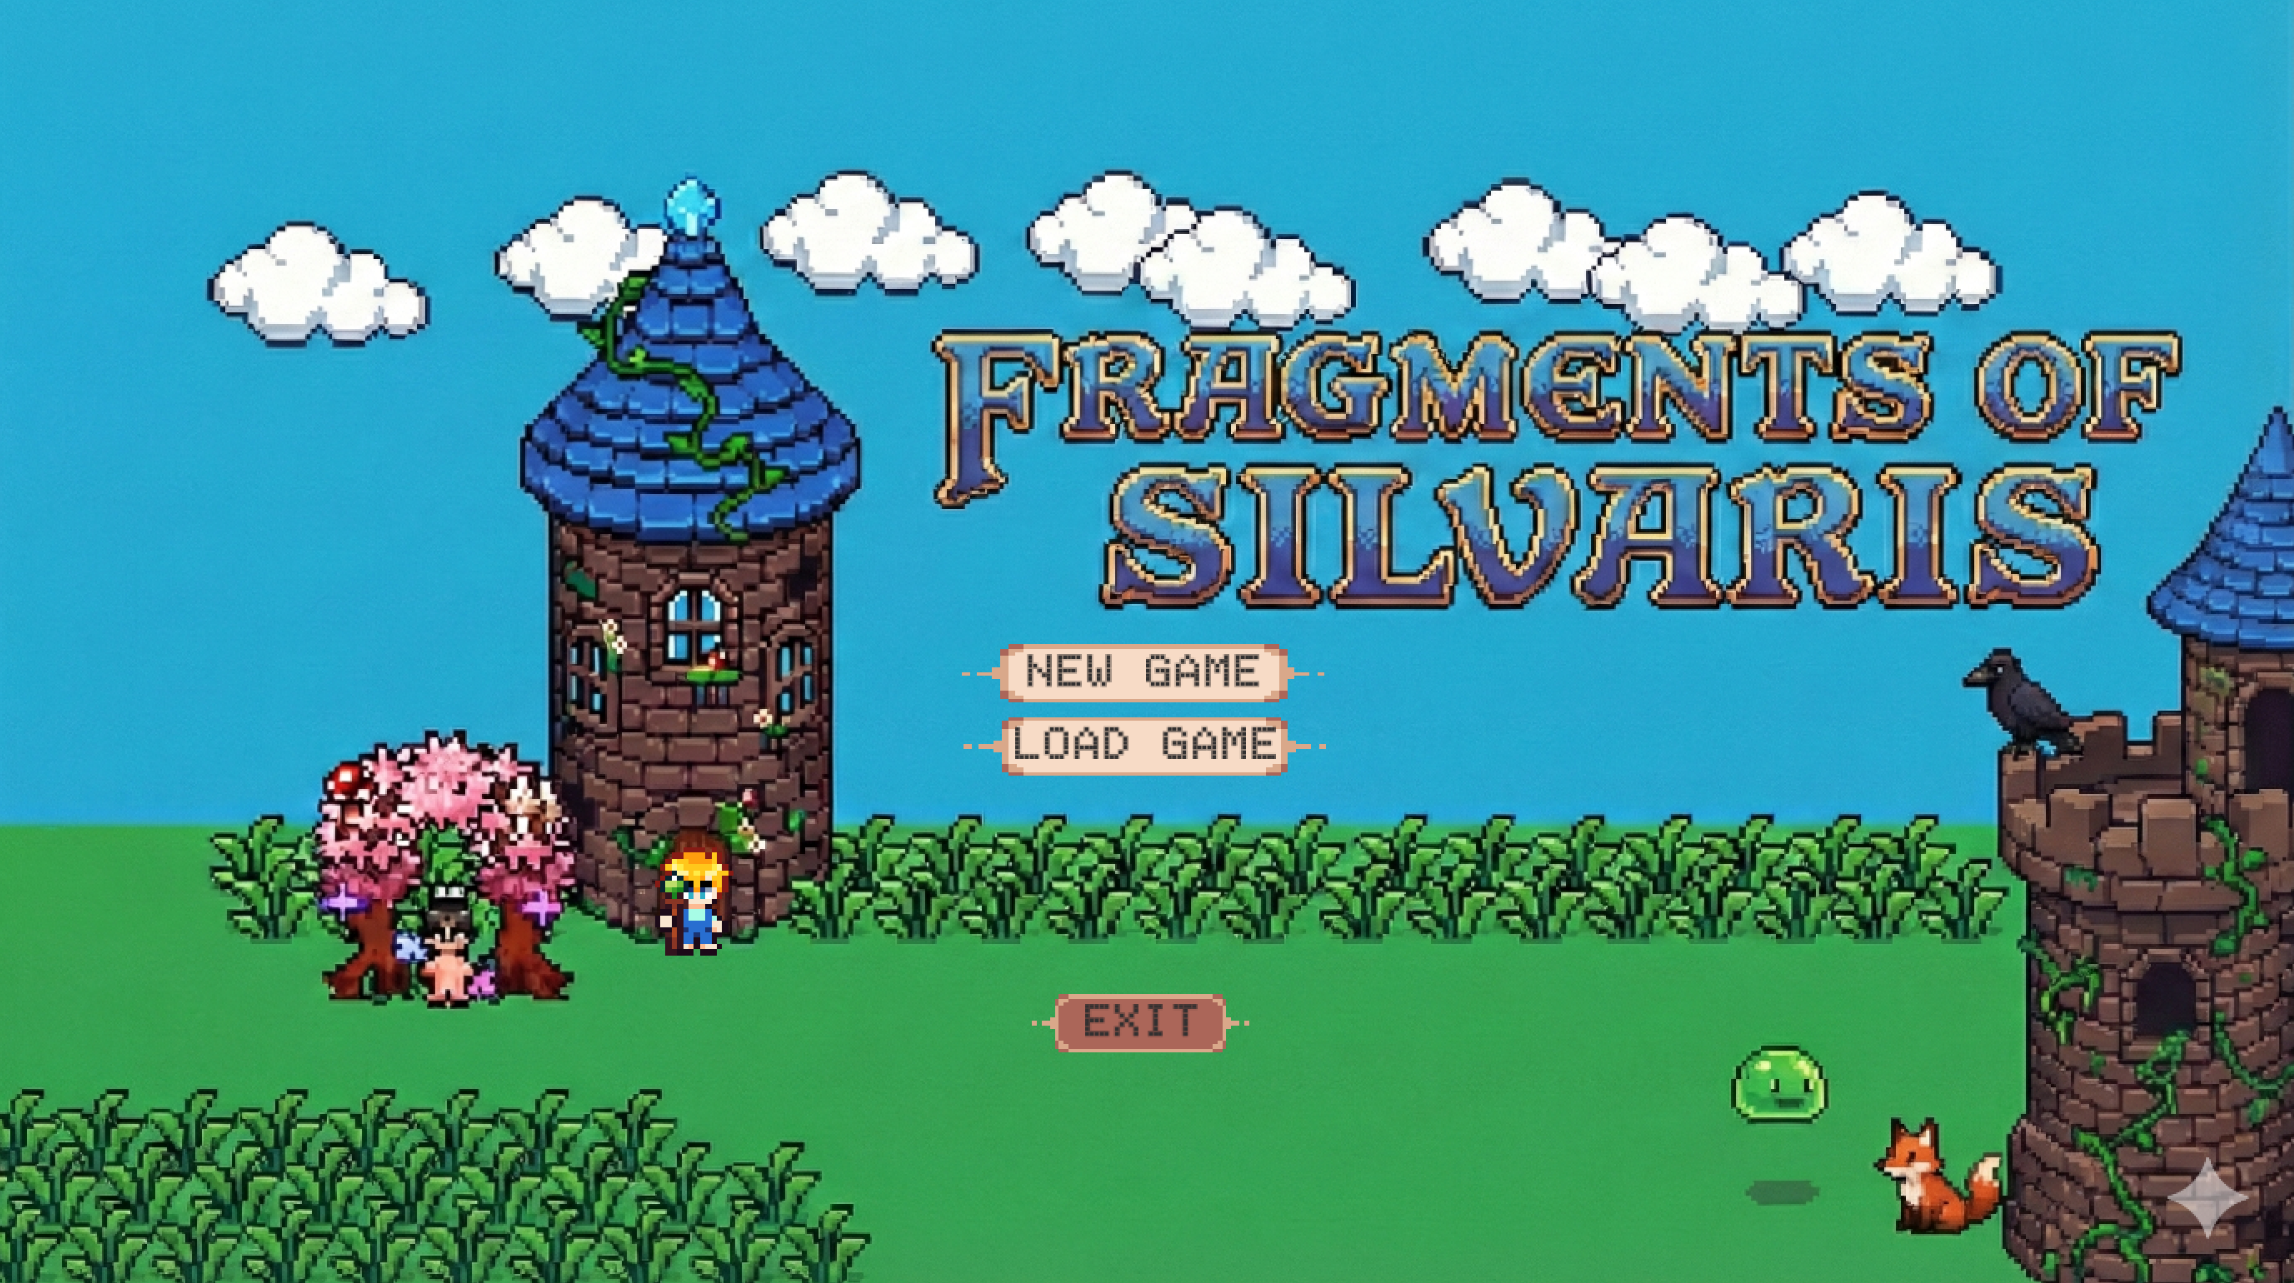
\includegraphics[width=0.8\textwidth]{Screenshot From 2026-02-11 19-06-40.png}
    \caption{Hauptmenü von Fragments of Silvaris}
    \label{fig:main_menu}
\end{figure}

\subsection{Spielziel}

Dein Ziel ist es, die Slime-Invasion zu stoppen, indem du:
\begin{itemize}
    \item Verschiedene Gebiete erkundest und von Gegnern befreist
    \item Deinen Charakter durch Kämpfe und Erfahrung verbesserst
    \item Mächtige Ausrüstung sammelst und ausrüstest
    \item Boss-Begegnungen meisterst
    \item Die Geschichte durch das Journal-System entdeckst
\end{itemize}

\subsection{Systemanforderungen}

\begin{itemize}
    \item \textbf{Plattform}: Windows/Linux PC
    \item \textbf{Empfohlene FPS}: Mindestens 60 \ac{FPS}
    \item \textbf{Steuerung}: Tastatur und Maus
\end{itemize}

% ============================================================================
% KAPITEL 2: SPIELSTART
% ============================================================================

\chapter{Spielstart und Einrichtung}

\section{Neues Spiel beginnen}

\subsection{Charakterauswahl}

Beim Start eines neuen Spiels wählst du einen von vier verschiedenen Charakter-Skins aus. Diese unterscheiden sich nur optisch -- alle haben die gleichen Startwerte.

\begin{figure}[H]
    \centering
    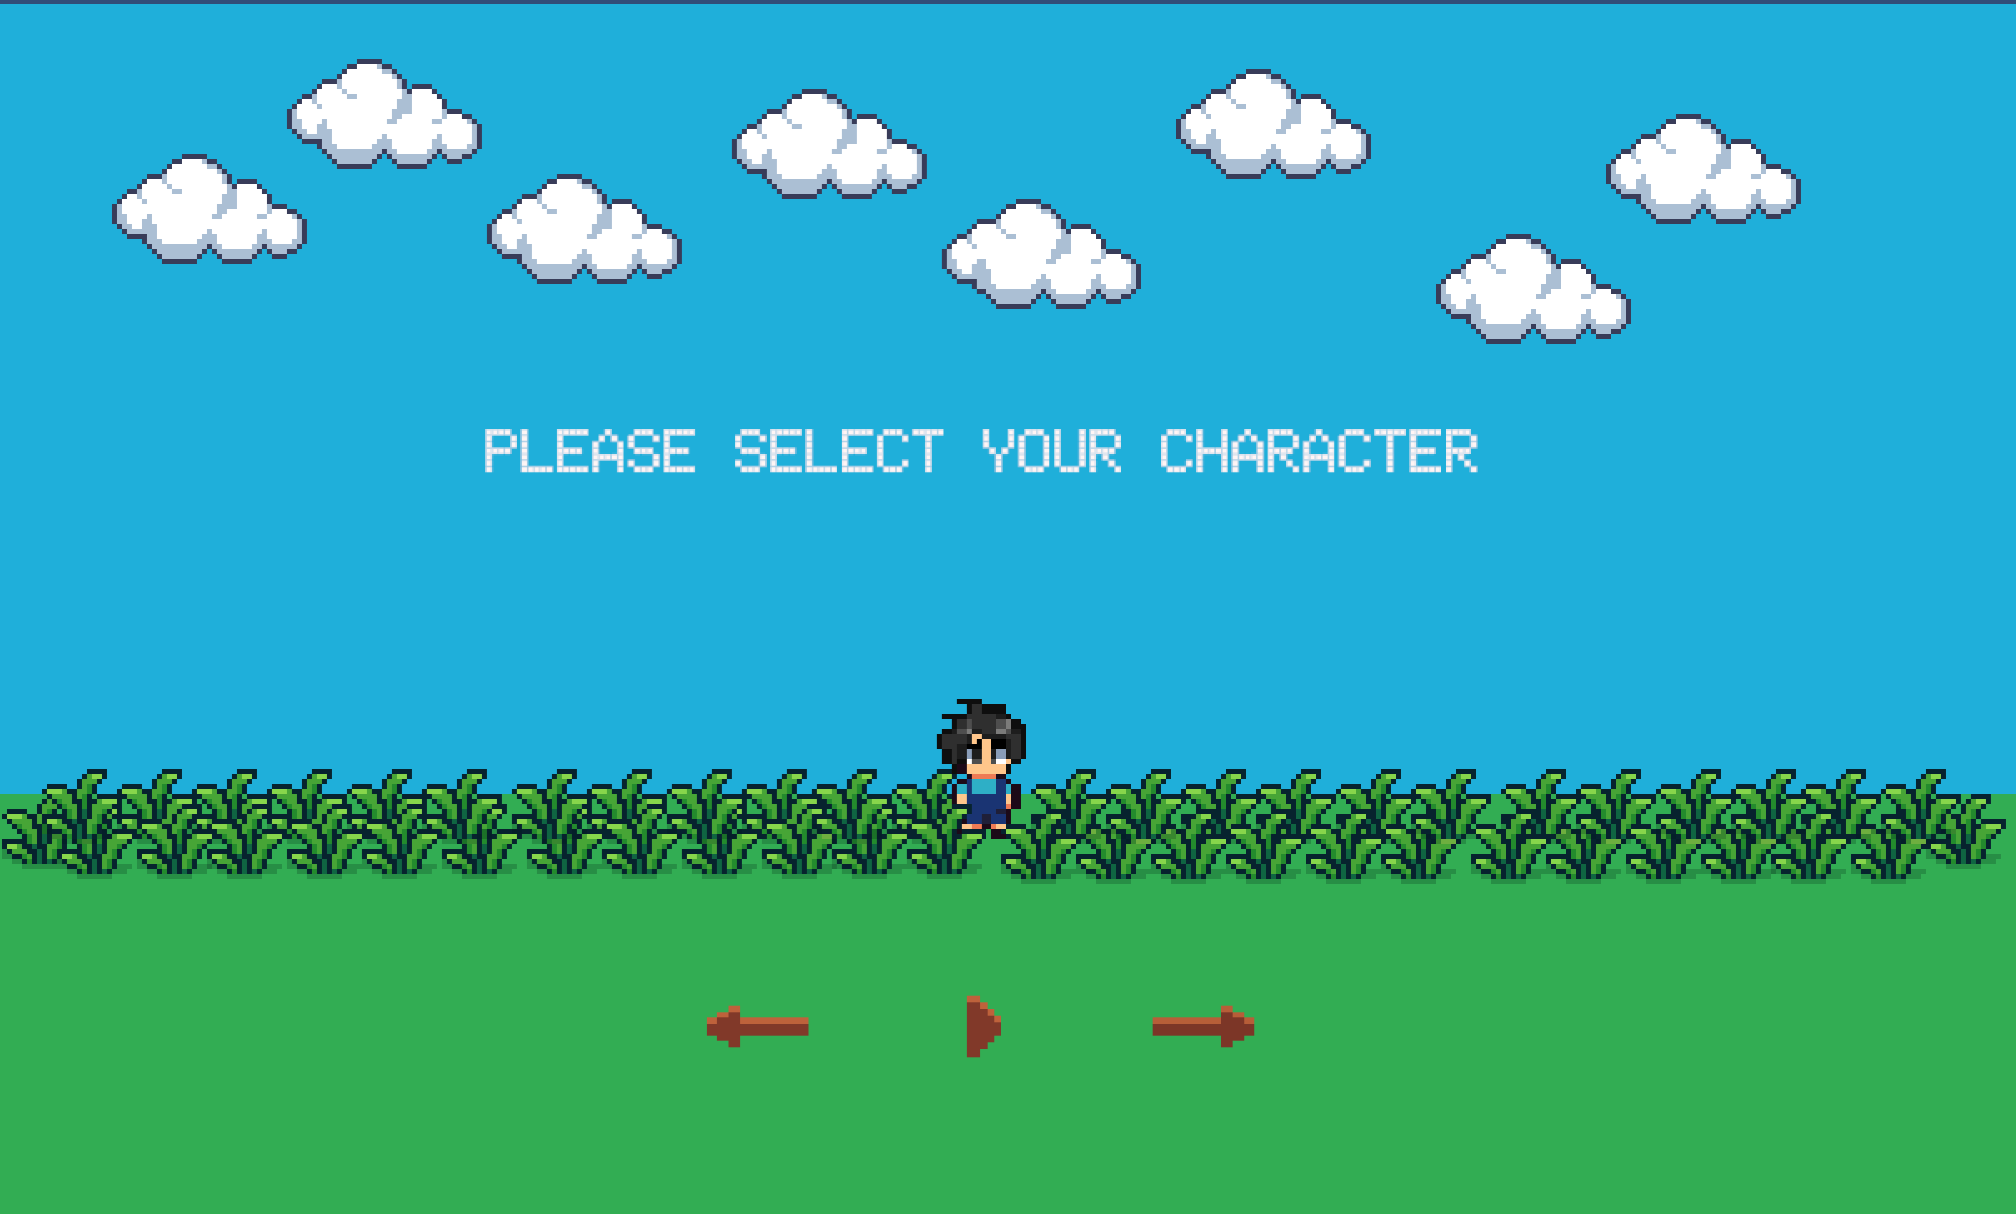
\includegraphics[width=0.7\textwidth]{Screenshot From 2026-02-11 19-07-01.png}
    \caption{Charakter-Auswahlbildschirm}
    \label{fig:character_select}
\end{figure}

\subsection{Hauptmenü}

Im Hauptmenü stehen dir folgende Optionen zur Verfügung:
\begin{itemize}
    \item \textbf{Neues Spiel}: Startet ein komplett neues Abenteuer
    \item \textbf{Spiel laden}: Lädt deinen letzten Spielstand
    \item \textbf{Einstellungen}: Passt Audio-Einstellungen an
    \item \textbf{Beenden}: Schließt das Spiel
\end{itemize}

\section{Speichern und Laden}

Das Spiel speichert deinen Fortschritt automatisch an wichtigen Punkten. Du kannst auch jederzeit über das Pause-Menü manuell speichern.

\textbf{Gespeicherte Daten umfassen}:
\begin{itemize}
    \item Charakter-Level und Statistiken
    \item Inventar und Ausrüstung
    \item Position in der Spielwelt
    \item Journal-Einträge und Story-Fortschritt
    \item Besiegte Gegner und gesammelte Items
\end{itemize}

% ============================================================================
% KAPITEL 3: STEUERUNG
% ============================================================================

\chapter{Steuerung}

\section{Grundlegende Steuerung}

\subsection{Bewegung}

\begin{table}[h]
\centering
\caption{Bewegungssteuerung}
\label{tab:movement_controls}
\begin{tabular}{|l|l|}
\hline
\textbf{Taste} & \textbf{Aktion} \\
\hline
W & Nach oben bewegen \\
A & Nach links bewegen \\
S & Nach unten bewegen \\
D & Nach rechts bewegen \\
\hline
\end{tabular}
\end{table}

Du kannst dich in 8 Richtungen bewegen, einschließlich diagonaler Bewegungen durch Kombination der Tasten (z.B. W+D für oben-rechts).

\subsection{Kampf}

\begin{table}[h]
\centering
\caption{Kampfsteuerung}
\label{tab:combat_controls}
\begin{tabular}{|l|l|}
\hline
\textbf{Eingabe} & \textbf{Aktion} \\
\hline
Linke Maustaste & Angriff in Mausrichtung \\
Mausbewegung & Zielrichtung für Angriffe \\
\hline
\end{tabular}
\end{table}

\textbf{Wichtig}: Deine Angriffe erfolgen immer in Richtung der Mausposition, nicht in Bewegungsrichtung!

\subsection{Menüs und Interfaces}

\begin{table}[h]
\centering
\caption{UI-Steuerung}
\label{tab:ui_controls}
\begin{tabular}{|l|l|}
\hline
\textbf{Taste} & \textbf{Aktion} \\
\hline
I & Inventar öffnen/schließen \\
E & Equipment-Bildschirm öffnen \\
M & Karte vergrößern/verkleinern \\
J & Journal öffnen/schließen \\
ESC & Pause-Menü öffnen \\
1-5 & Hotbar-Items verwenden \\
\hline
\end{tabular}
\end{table}

% ============================================================================
% KAPITEL 4: SPIELMECHANIKEN
% ============================================================================

\chapter{Spielmechaniken}

\section{Kampfsystem}

\subsection{Angriffe ausführen}

Dein Charakter führt Nahkampf-Angriffe aus, die in einem 60°-Kegel vor dir treffen:

\begin{itemize}
    \item \textbf{Reichweite}: 2.0 Einheiten
    \item \textbf{Angriffswinkel}: 60° Kegel (30° links + 30° rechts von der Angriffsrichtung)
    \item \textbf{Attackengeschwindigkeit}: Bis zu 2 Angriffe pro Sekunde
    \item \textbf{Multi-Target}: Du kannst mehrere Gegner gleichzeitig treffen
\end{itemize}

\subsection{Schaden und Verteidigung}

\textbf{Schadenberechnung}:
\begin{itemize}
    \item Dein Basis-Schaden hängt von deinem Level ab
    \item Waffen und Ausrüstung erhöhen deinen Schaden
    \item Kritische Treffer können mit erhöhter Chance und Multiplikator auftreten
\end{itemize}

\textbf{Verteidigung}:
\begin{itemize}
    \item Rüstungsteile erhöhen deine Verteidigung
    \item Die Verteidigung reduziert eingehenden Schaden
    \item Maximum 80\% Schadensreduktion möglich
    \item Mindestens 1 Schadenspunkt wird immer durchkommen
\end{itemize}

\subsection{Gegner-Verhalten}

Slime-Gegner haben unterschiedliche Eigenschaften:

\begin{itemize}
    \item \textbf{Blue Slime}: Hohe Verteidigung, defensiv
    \item \textbf{Green Slime}: Ausgewogene Standardgegner
    \item \textbf{Red Slime}: Hoher Schaden, aggressiv
    \item \textbf{Yellow Slime}: Schnelle Bewegung
\end{itemize}

\begin{figure}[H]
    \centering
    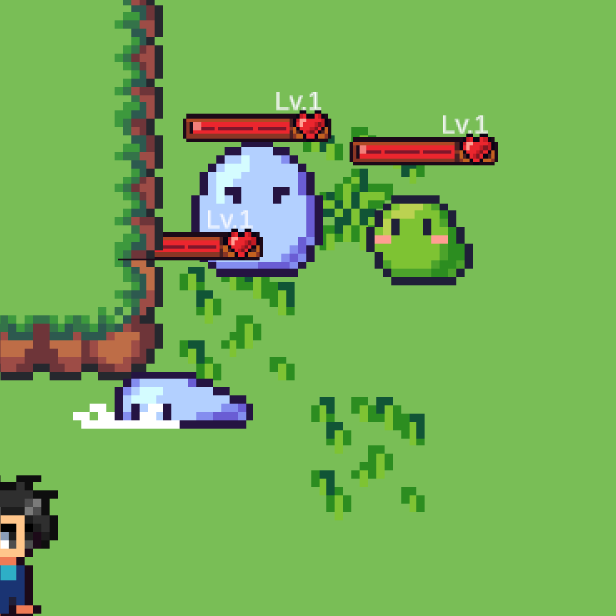
\includegraphics[width=0.5\textwidth]{Screenshot From 2026-02-11 19-11-59.png}
    \caption{Verschiedene Slime-Typen mit Healthbars}
    \label{fig:slimes}
\end{figure}

\textbf{Gegner-KI}:
\begin{itemize}
    \item Gegner erkennen dich in einem bestimmten Radius (ca. 5 Einheiten)
    \item Sie verfolgen dich und weichen Hindernissen intelligent aus
    \item Vor einem Angriff gibt es eine kurze "Telegraph"-Phase -- nutze diese Zeit zum Ausweichen!
\end{itemize}

\section{Progression und Levelaufstieg}

\subsection{Erfahrungspunkte sammeln}

Du erhältst \ac{XP} durch:
\begin{itemize}
    \item Besiegen von Gegnern (20 XP + Level-Bonus)
    \item Abschließen von Boss-Encounters
\end{itemize}

\subsection{Levelaufstieg}

Bei jedem Levelaufstieg:
\begin{itemize}
    \item Erhöht sich deine maximale \ac{HP} (Gesundheit)
    \item Steigt dein maximales \ac{MP} (Mana)
    \item Wächst dein Basis-Schaden
    \item Werden \ac{HP} und \ac{MP} vollständig aufgefüllt
\end{itemize}

Die benötigten \ac{XP} für den nächsten Level steigen exponentiell an (Faktor 1.5).

\subsection{Charakter-Statistiken}

\begin{table}[h]
\centering
\caption{Charakter-Statistiken}
\label{tab:stats}
\begin{tabular}{|l|p{8cm}|}
\hline
\textbf{Stat} & \textbf{Beschreibung} \\
\hline
HP & Gesundheitspunkte -- bei 0 HP ist das Spiel vorbei \\
MP & Manapunkte -- für zukünftige Fähigkeiten reserviert \\
DMG & Schaden pro Angriff \\
DEF & Verteidigung -- reduziert eingehenden Schaden \\
Krit-Quote & Wahrscheinlichkeit für kritische Treffer \\
Krit-Schaden & Schadens-Multiplikator bei kritischen Treffern \\
\hline
\end{tabular}
\end{table}

\section{Inventar und Ausrüstung}

\subsection{Inventar-System}

Das Inventar bietet 49 Slots (7x7 Raster) für Items:
\begin{itemize}
    \item \textbf{Ausrüstung}: Waffen, Rüstungen, Accessoires
    \item \textbf{Verbrauchsgegenstände}: Tränke (HP, MP, Buffs)
    \item \textbf{Quest-Items}: Story-relevante Gegenstände
\end{itemize}

\subsection{Ausrüstungsplätze}

Es gibt 6 Ausrüstungsplätze:
\begin{enumerate}
    \item \textbf{Waffe}: Erhöht deinen Schaden
    \item \textbf{Helm}: Bietet Verteidigung
    \item \textbf{Rüstung}: Hauptverteidigungsquelle
    \item \textbf{Stiefel}: Verteidigung und möglicherweise Geschwindigkeitsboni
    \item \textbf{Handschuhe}: Verteidigung und Schadensboni
    \item \textbf{Accessoire}: Spezielle Boni (Krit-Chance, Stats, etc.)
\end{enumerate}

\textbf{Items ausrüsten}:
\begin{itemize}
    \item Öffne das Equipment-Menü mit \textbf{E}
    \item Ziehe Items per Drag-and-Drop auf die entsprechenden Slots
    \item Ausgerüstete Items werden sofort wirksam
\end{itemize}

\subsection{Hotbar}

Die Hotbar am unteren Bildschirmrand bietet 5 Schnellzugriff-Slots:
\begin{itemize}
    \item Ziehe Items (meist Tränke) aus dem Inventar in die Hotbar
    \item Verwende Hotbar-Items mit den Tasten \textbf{1-5}
    \item Besonders nützlich für Heiltränke im Kampf!
\end{itemize}

\section{Gold und Handel}

\subsection{Gold verdienen}

Gold erhältst du durch:
\begin{itemize}
    \item Besiegen von Gegnern (zufällige Drops)
    \item Verkauf von Items an Händler
    \item Finden von Truhen
\end{itemize}

\subsection{Shop-System}

In Dörfern findest du Händler-\acp{NPC}:

\begin{figure}[H]
    \centering
    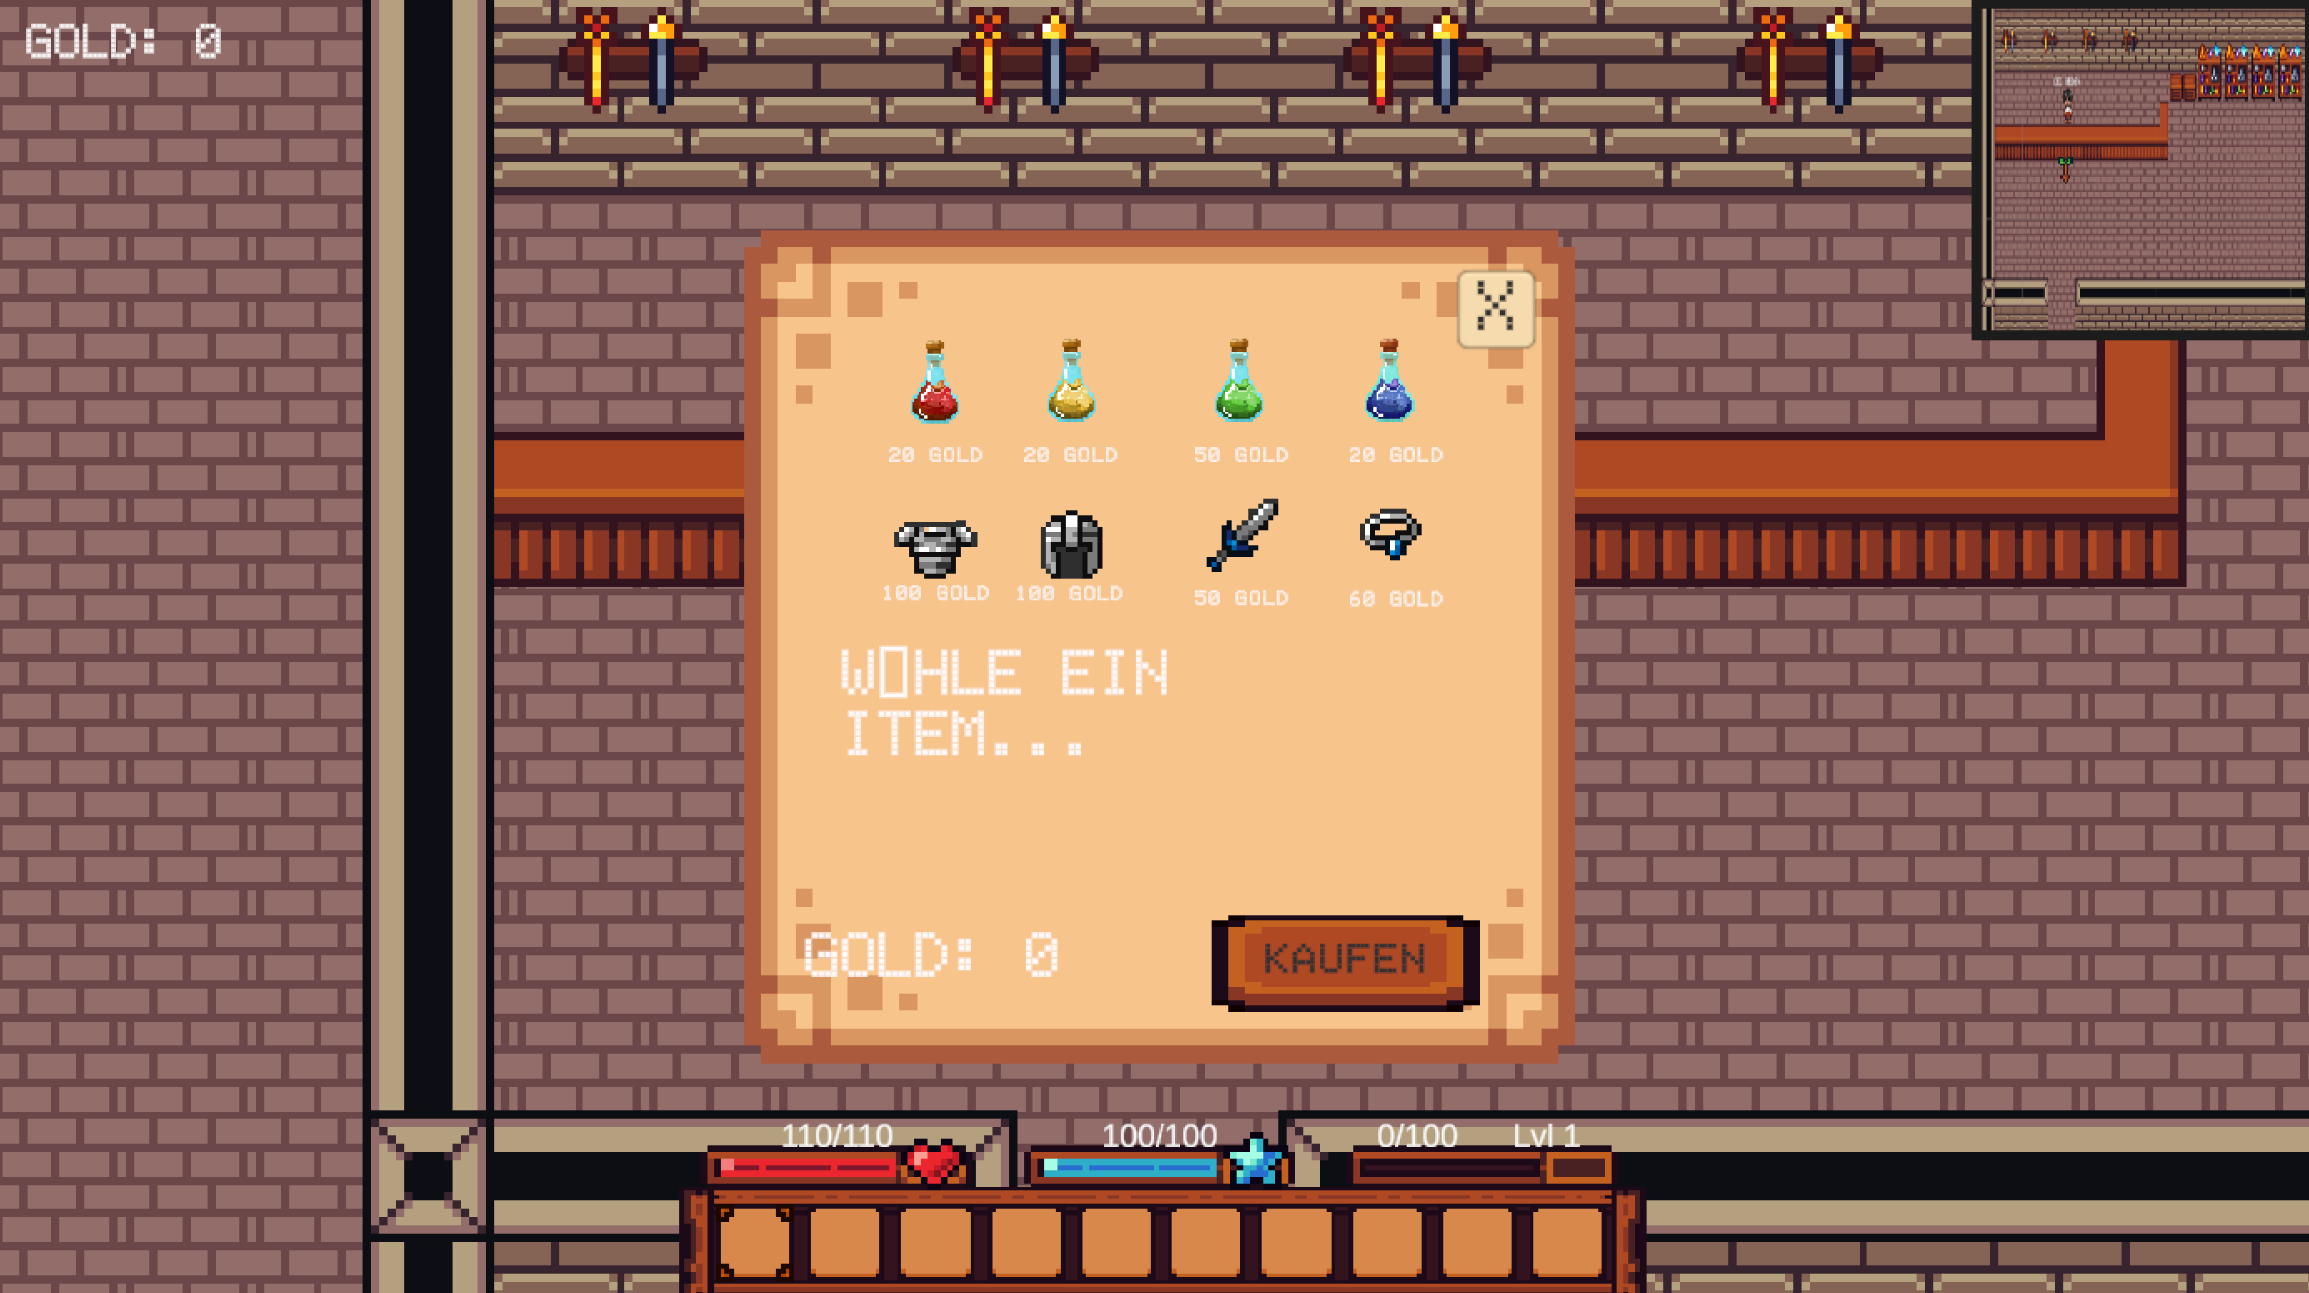
\includegraphics[width=0.7\textwidth]{Screenshot From 2026-02-11 19-17-05.png}
    \caption{Shop-Interface mit verfügbaren Items}
    \label{fig:shop}
\end{figure}

\textbf{Im Shop kannst du}:
\begin{itemize}
    \item Items kaufen (Waffen, Rüstungen, Tränke)
    \item Eigene Items verkaufen
    \item Preise vergleichen
\end{itemize}

% ============================================================================
% KAPITEL 5: SPIELWELT
% ============================================================================

\chapter{Die Spielwelt}

\section{Weltenaufbau}

Das Spiel besteht aus 10 miteinander verbundenen Bereichen:
\begin{itemize}
    \item \textbf{Heimatbasis}: Dein Ausgangspunkt
    \item \textbf{3 Dörfer}: Sichere Zonen mit \acp{NPC} und Händlern
    \item \textbf{3 Wildnisgebiete}: Gefährliche Zonen voller Gegner
    \item \textbf{2 Boss-Arenen}: Spezielle Bereiche für Boss-Kämpfe
\end{itemize}

\section{Navigation}

\subsection{Minimap}

Die Minimap oben links zeigt:
\begin{itemize}
    \item Deine aktuelle Position (weißer Punkt)
    \item Die Umgebung
    \item Wichtige Orientierungspunkte
\end{itemize}

\begin{figure}[H]
    \centering
    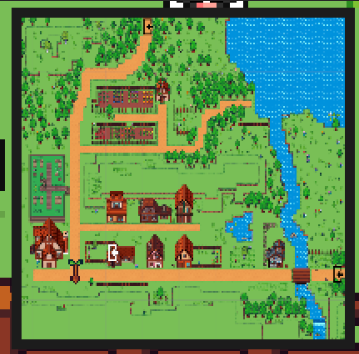
\includegraphics[width=0.3\textwidth]{Screenshot From 2026-02-11 19-11-14.png}
    \caption{Minimap-Ansicht}
    \label{fig:minimap}
\end{figure}

\subsection{Karten-Zoom}

Drücke \textbf{M} für eine vergrößerte Kartenansicht mit detaillierter Übersicht des gesamten Gebiets.

\begin{figure}[H]
    \centering
    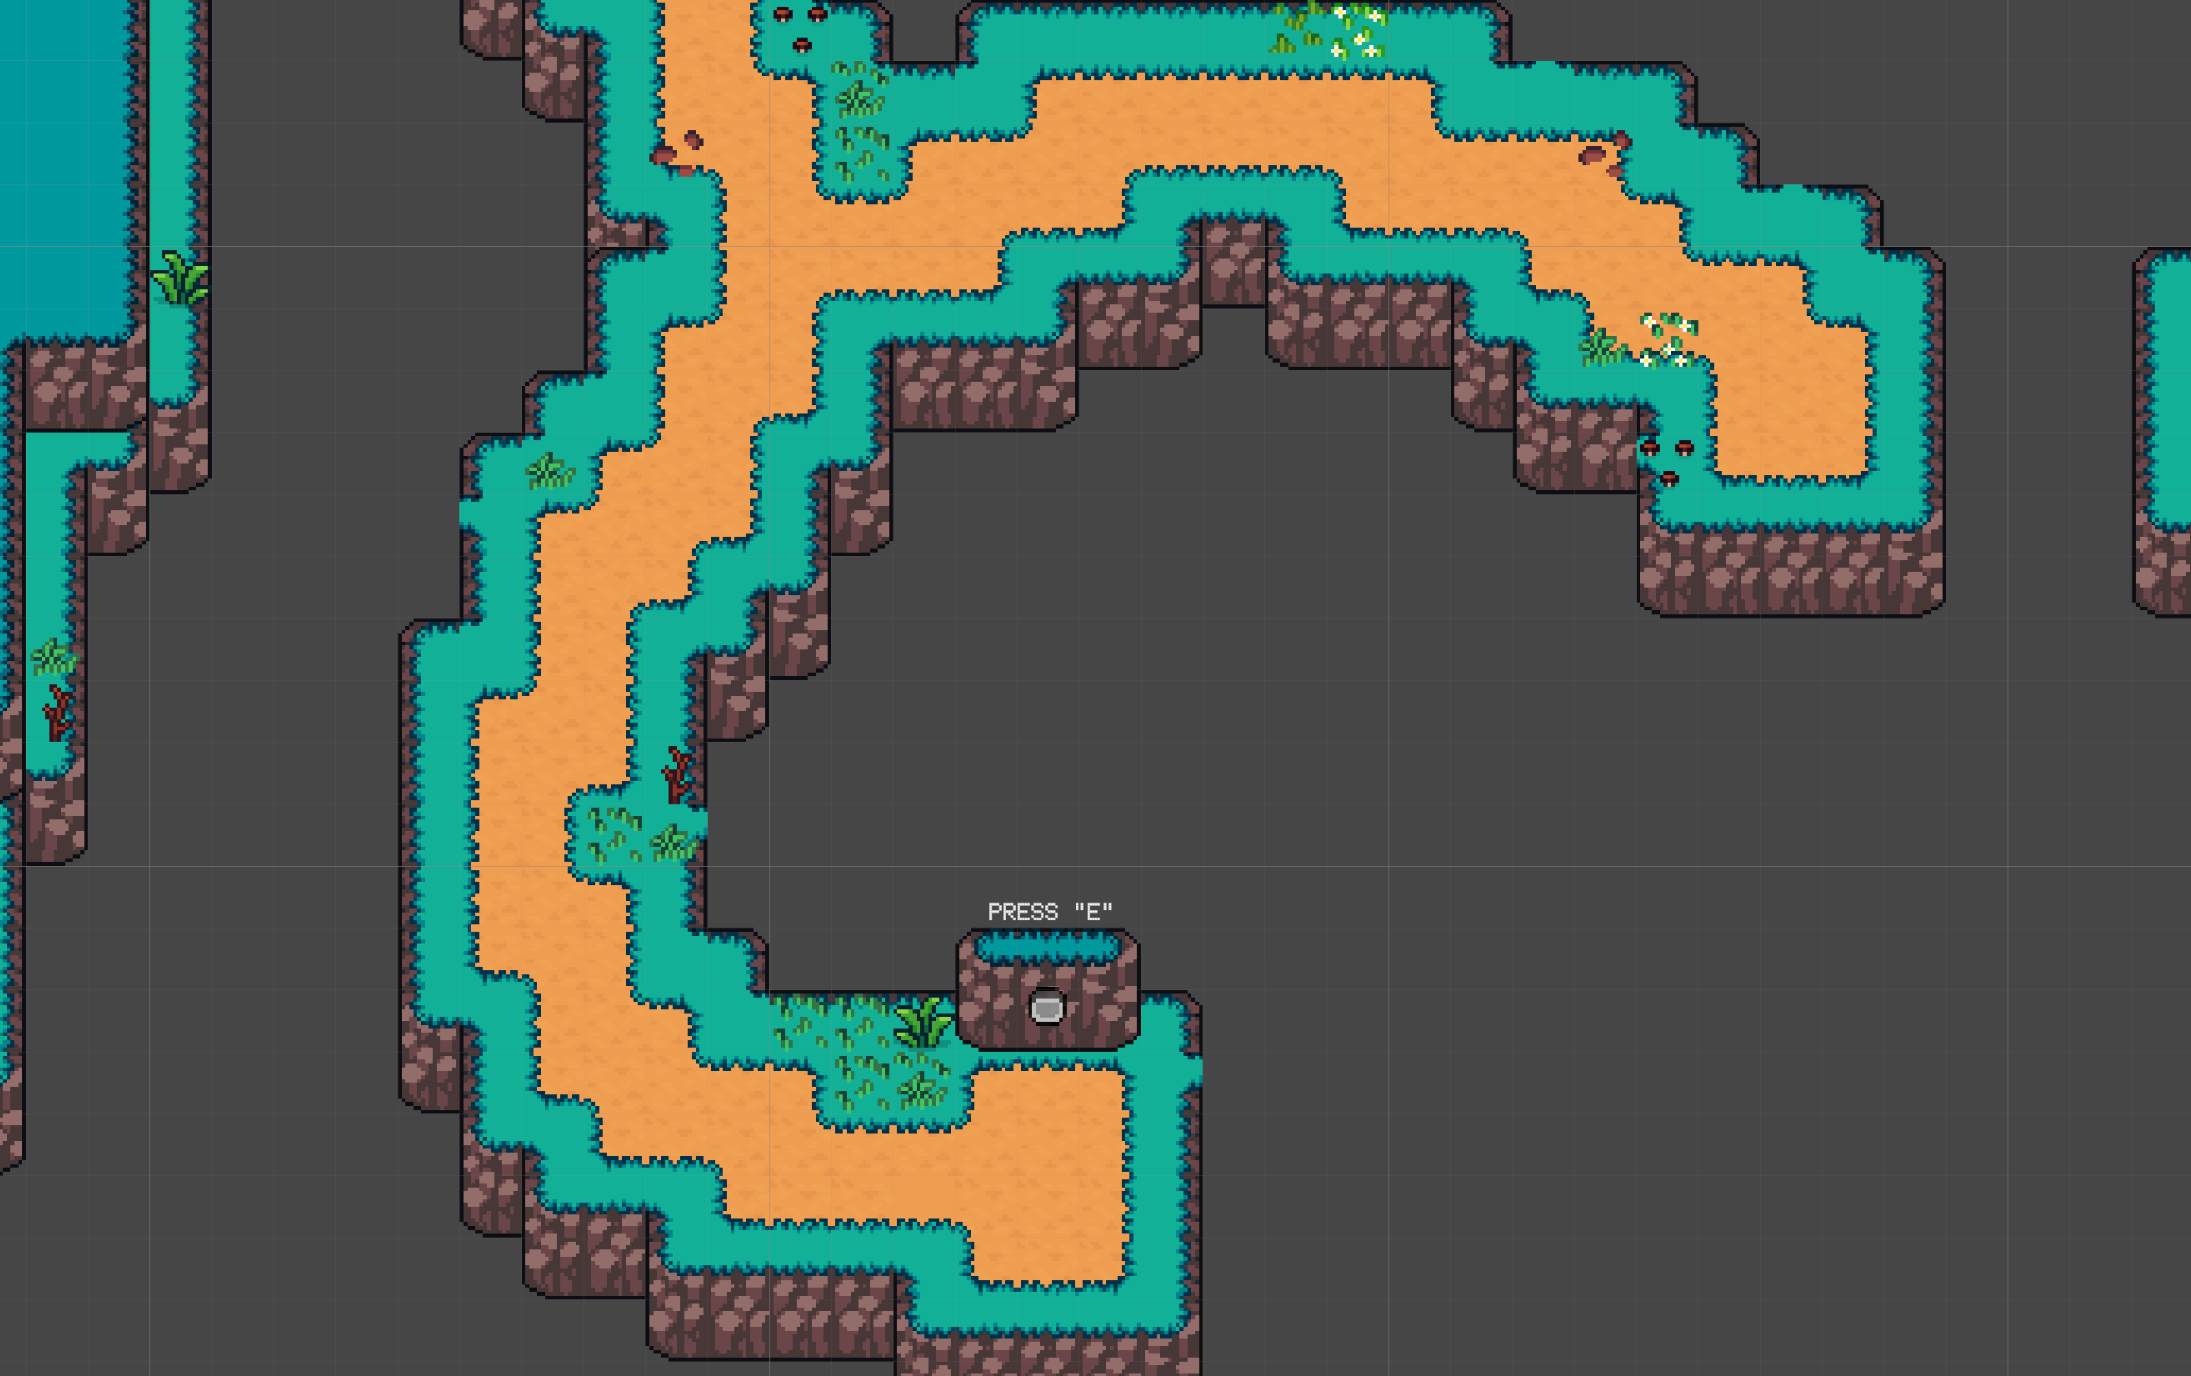
\includegraphics[width=0.7\textwidth]{Screenshot From 2026-02-11 19-21-57.png}
    \caption{Gezoomte Kartenansicht}
    \label{fig:map_zoom}
\end{figure}

\subsection{Szenenübergänge}

Bereiche sind über Trigger-Zonen verbunden:
\begin{itemize}
    \item Gehe zu Ausgängen am Rand der Karte
    \item Ein Loading-Screen erscheint kurz
    \item Du spawst am entsprechenden Eingang des neuen Bereichs
\end{itemize}

\section{Interaktive Elemente}

\subsection{NPCs}

In Dörfern triffst du auf freundliche \acp{NPC}:

\begin{figure}[H]
    \centering
    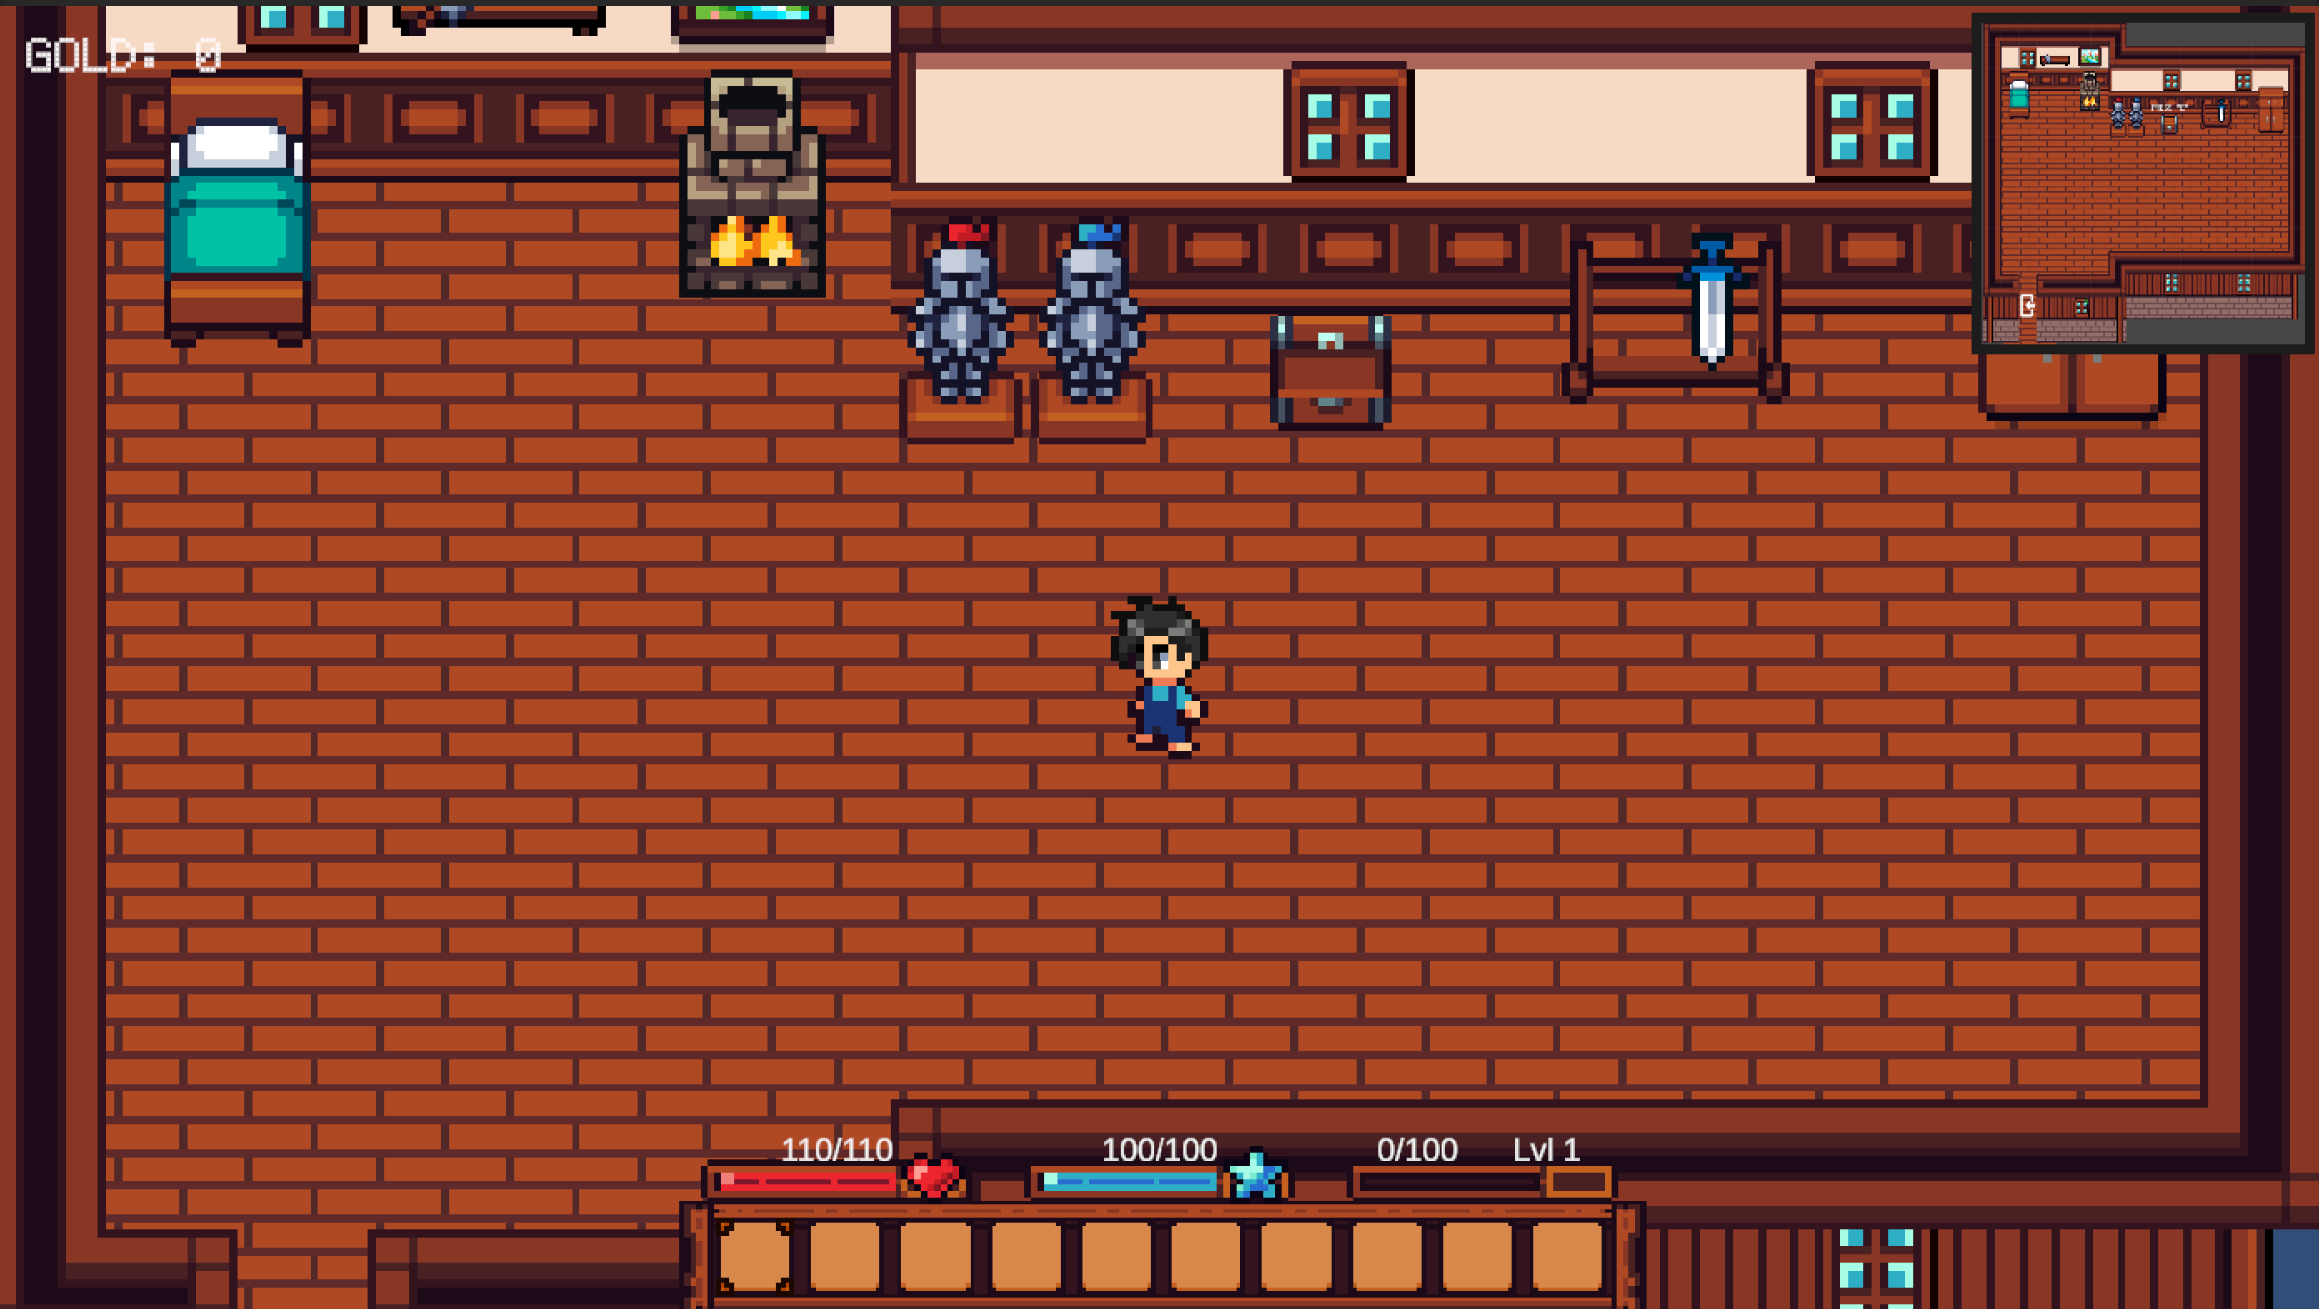
\includegraphics[width=0.6\textwidth]{Screenshot From 2026-02-11 19-10-05.png}
    \caption{\acp{NPC} in einem Gebäude}
    \label{fig:npcs}
\end{figure}

\textbf{NPC-Typen}:
\begin{itemize}
    \item \textbf{Wandernde NPCs}: Bewohner, die herumgehen
    \item \textbf{Händler}: Verkaufen und kaufen Items
    \item \textbf{Quest-Geber}: Zukünftige Erweiterung
\end{itemize}

\subsection{Truhen (Chests)}

Versteckte Truhen enthalten Story-Fragmente:

\begin{figure}[H]
    \centering
    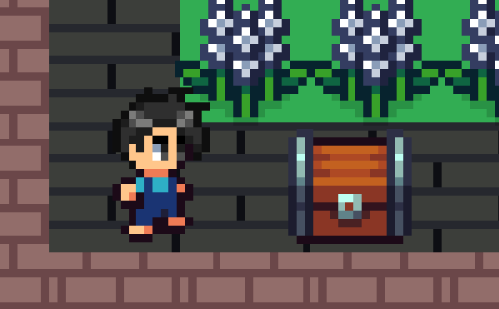
\includegraphics[width=0.4\textwidth]{Screenshot From 2026-02-11 19-16-03.png}
    \caption{Eine findbare Truhe}
    \label{fig:chest}
\end{figure}

\begin{itemize}
    \item Suche in verschiedenen Szenen nach Truhen
    \item Jede Truhe enthält einen Teil der Hintergrundgeschichte
    \item Finde alle Truhen, um die vollständige Story zu enthüllen!
\end{itemize}

\subsection{Ambiente-Elemente}

Die Welt ist bevölkert von:
\begin{itemize}
    \item \textbf{Tieren}: Kühe und Raben beleben die Landschaft
    \item \textbf{Vegetation}: Bäume, Blumen und Gras
    \item \textbf{Gebäuden}: Häuser, Läden und andere Strukturen
\end{itemize}

\begin{figure}[H]
    \centering
    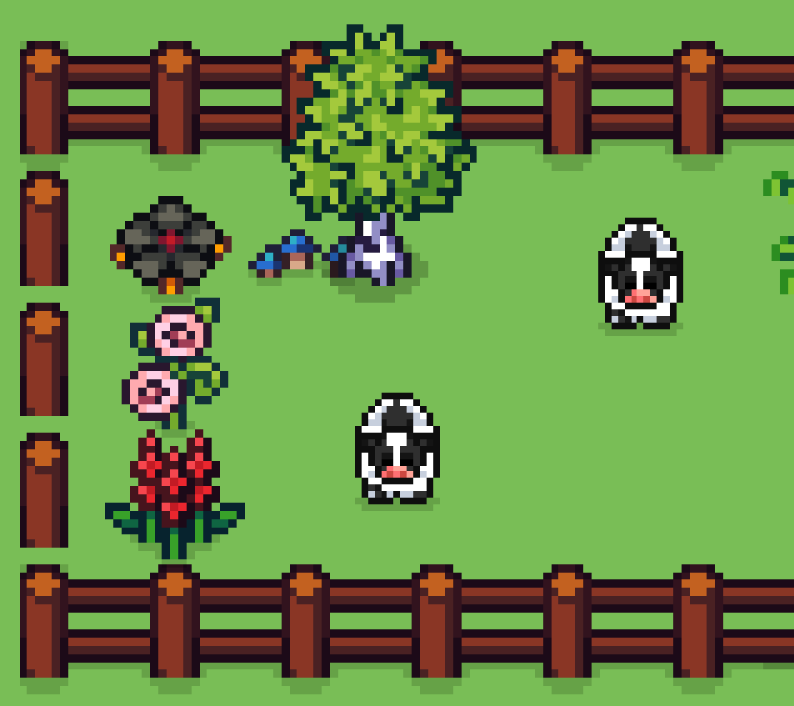
\includegraphics[width=0.6\textwidth]{Screenshot From 2026-02-11 19-12-26.png}
    \caption{Ambiente-Elemente: Kühe und Raben}
    \label{fig:ambient}
\end{figure}

% ============================================================================
% KAPITEL 6: BENUTZEROBERFLÄCHE
% ============================================================================

\chapter{Benutzeroberfläche (UI)}

\section{HUD-Elemente}

\subsection{Ressourcen-Balken (oben links)}

\begin{itemize}
    \item \textbf{Roter Balken}: Gesundheit (\ac{HP})
    \item \textbf{Blauer Balken}: Mana (\ac{MP})
    \item \textbf{Gelber Balken}: Ausdauer (Stamina)
\end{itemize}

Jeder Balken zeigt den aktuellen Wert und das Maximum an.

\subsection{Erfahrungsbalken}

Am unteren Bildschirmrand siehst du:
\begin{itemize}
    \item Dein aktuelles Level
    \item Fortschritt zum nächsten Level (als Balken)
    \item Aktuelle und benötigte \ac{XP}
\end{itemize}

\subsection{Gold-Anzeige}

Die Goldanzeige zeigt dein aktuelles Vermögen. Achte darauf, genug Gold für wichtige Käufe zu sparen!

\section{Menüs}

\subsection{Inventar-Menü (I)}

\begin{itemize}
    \item 7x7 Raster mit 49 Slots
    \item Drag-and-Drop zum Verschieben
    \item Rechtsklick für Item-Aktionen
    \item Gewichts- oder Slot-basierte Limitierung
\end{itemize}

\subsection{Equipment-Menü (E)}

\begin{itemize}
    \item Zeigt alle 6 Ausrüstungsslots
    \item Zeigt deine aktuellen Statistiken
    \item Vergleiche neue Items mit ausgerüsteten
\end{itemize}

\subsection{Journal (J)}

Das Journal enthält Story-Einträge, die freigeschaltet werden durch:
\begin{itemize}
    \item Erreichen bestimmter Bereiche
    \item Besiegen einer bestimmten Anzahl Gegner
    \item Level-Meilensteine
    \item Boss-Siege
    \item Finden von Truhen
\end{itemize}

Lies das Journal, um die Hintergrundgeschichte zu verstehen!

\subsection{Pause-Menü (ESC)}

\begin{figure}[H]
    \centering
    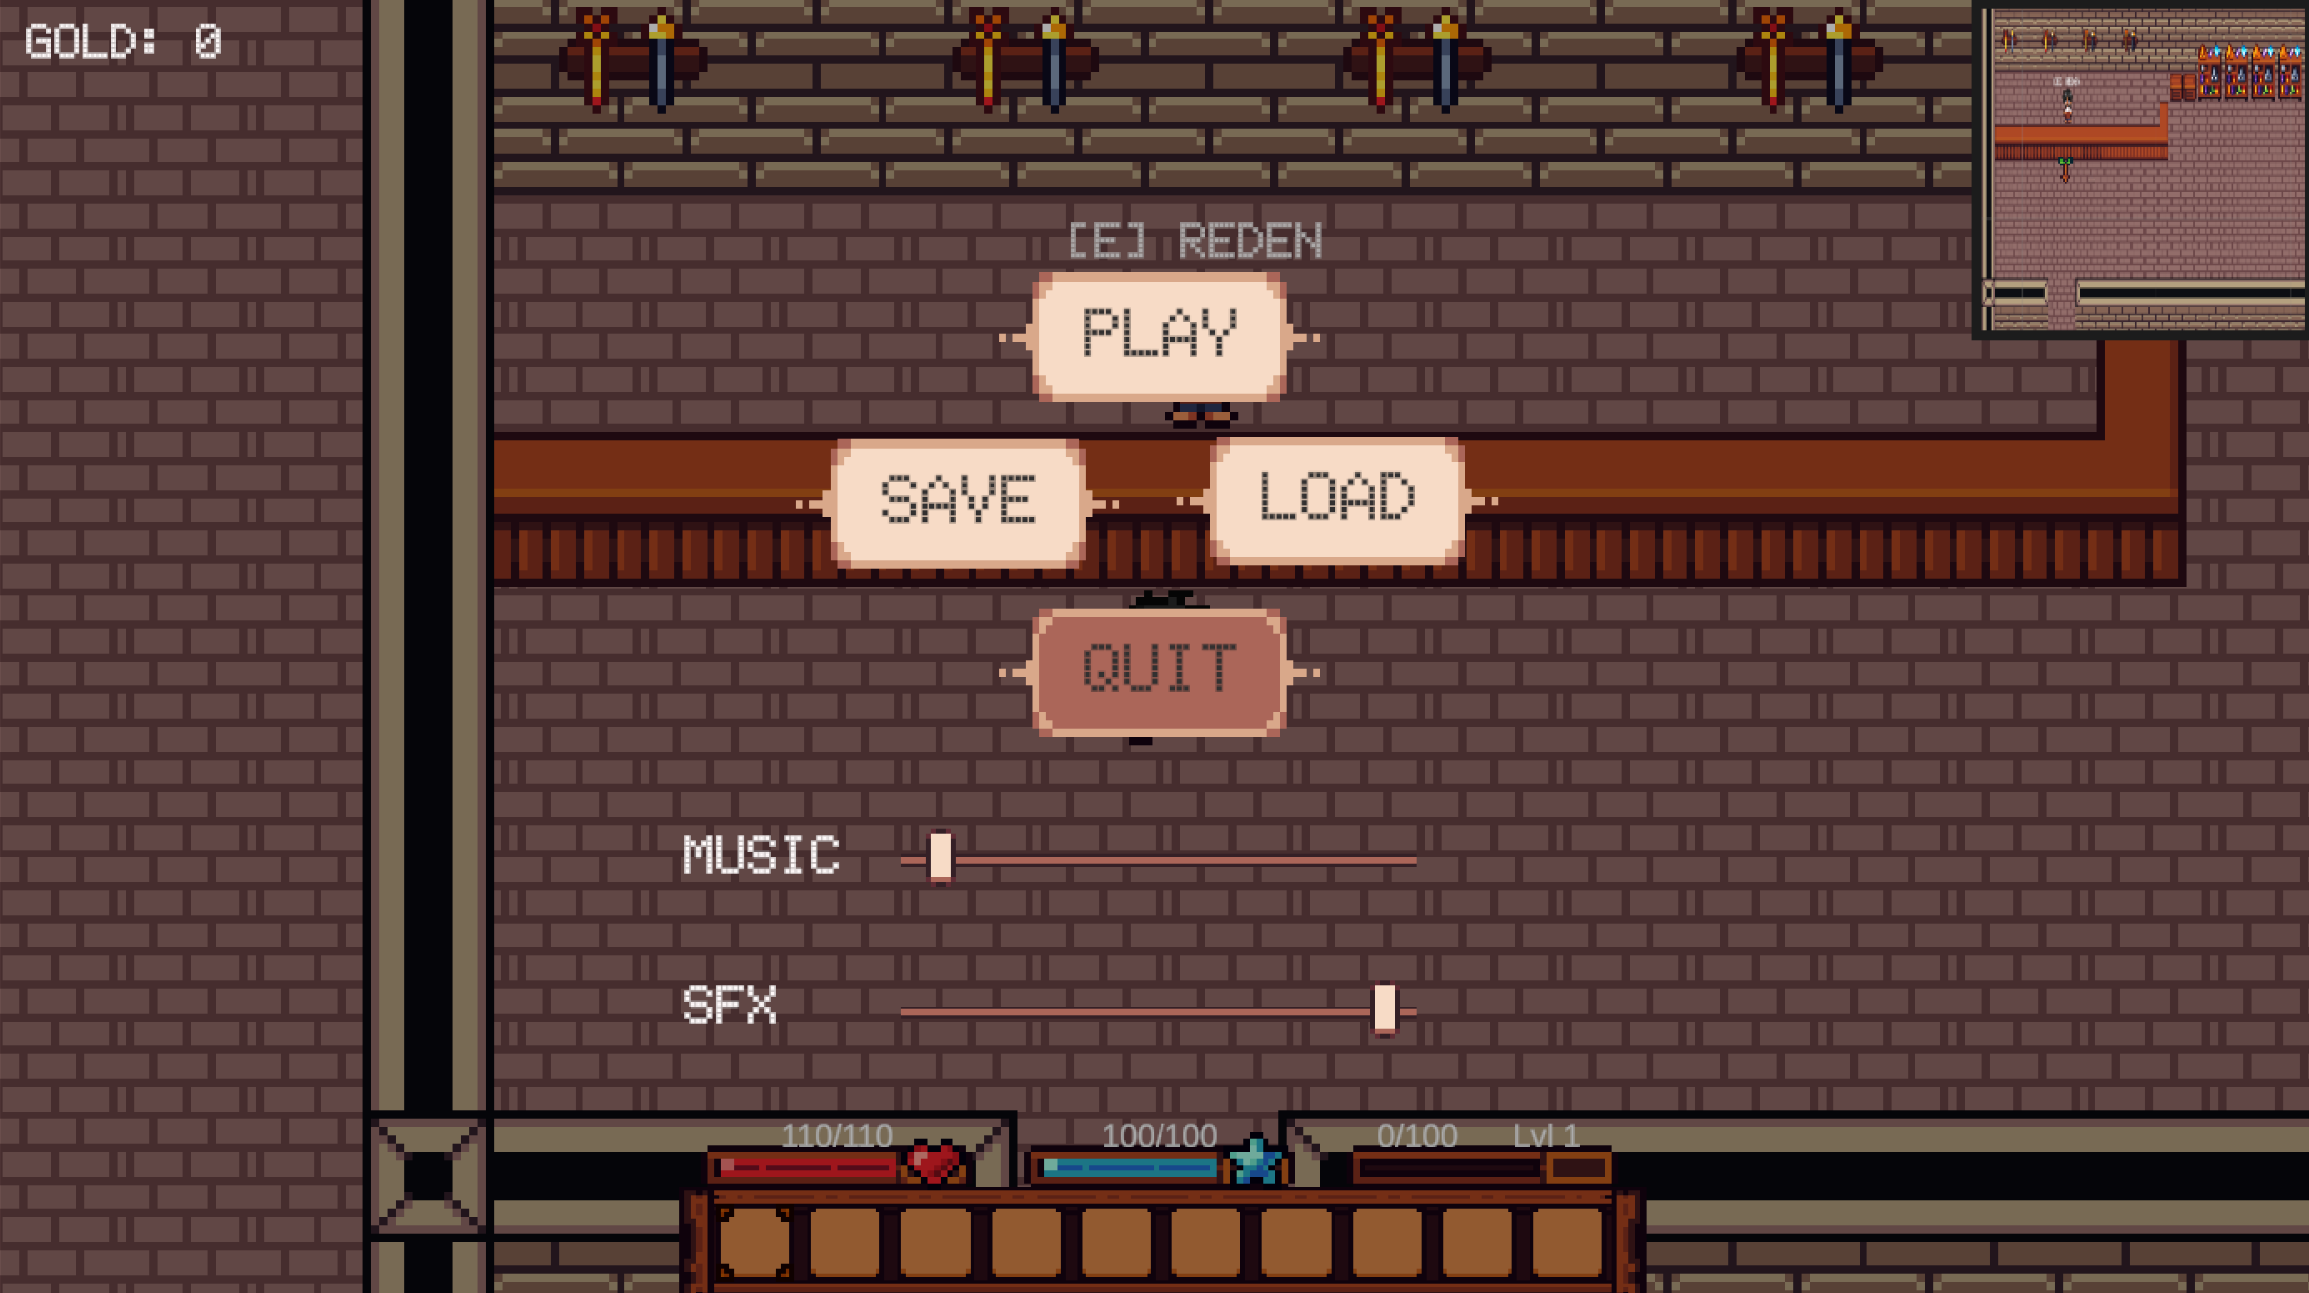
\includegraphics[width=0.7\textwidth]{Screenshot From 2026-02-11 19-16-48.png}
    \caption{Pause-Menü mit Einstellungen}
    \label{fig:pause}
\end{figure}

Im Pause-Menü kannst du:
\begin{itemize}
    \item Das Spiel fortsetzen
    \item Lautstärke anpassen (Musik, Sound Effects)
    \item Speichern
    \item Zum Hauptmenü zurückkehren
    \item Das Spiel beenden
\end{itemize}

% ============================================================================
% KAPITEL 7: SPIELTIPPS UND STRATEGIEN
% ============================================================================

\chapter{Spieltipps und Strategien}

\section{Für Anfänger}

\subsection{Grundlegende Tipps}

\begin{enumerate}
    \item \textbf{Nutze die Telegraph-Phase}: Gegner zeigen ihre Angriffe kurz vorher an -- weiche in dieser Zeit aus!

    \item \textbf{Heile regelmäßig}: Kaufe Heiltränke und lege sie auf die Hotbar (1-5) für schnellen Zugriff

    \item \textbf{Erkunde gründlich}: Truhen enthalten wichtige Story-Informationen

    \item \textbf{Verbessere deine Ausrüstung}: Besuche Händler regelmäßig und kaufe bessere Ausrüstung

    \item \textbf{Spare Gold}: Nicht jedes Item ist es wert gekauft zu werden -- priorisiere Waffen und Rüstungen
\end{enumerate}

\subsection{Kampf-Tipps}

\begin{itemize}
    \item \textbf{Positionierung ist wichtig}: Versuche, mehrere Gegner gleichzeitig in deinem Angriffskegel zu treffen

    \item \textbf{Kite die Gegner}: Bewege dich rückwärts während du angreifst, um Schaden zu vermeiden

    \item \textbf{Nutze die Umgebung}: Hindernisse können dir helfen, Gegner zu channeln

    \item \textbf{Achte auf deine \ac{HP}}: Heile, bevor du bei niedriger Gesundheit bist
\end{itemize}

\section{Fortgeschrittene Strategien}

\subsection{Effizientes Leveln}

\begin{itemize}
    \item Konzentriere dich auf Gegner nahe deinem Level
    \item Boss-Encounters geben viel \ac{XP} -- nutze sie!
    \item Zu niedrig-levelige Gegner geben kaum \ac{XP}
\end{itemize}

\subsection{Goldfarming}

\begin{itemize}
    \item Verkaufe überflüssige Ausrüstung
    \item Gegner in höheren Levelbereichen droppen mehr Gold
    \item Spare für die besten Ausrüstungsteile
\end{itemize}

\subsection{Boss-Kämpfe meistern}

Boss-Encounters sind besondere Herausforderungen:
\begin{itemize}
    \item \textbf{Vorbereitung}: Stelle sicher, dass du volle \ac{HP} hast und Heiltränke dabei sind
    \item \textbf{Level-Vorteil}: Boss-Slimes sind 3 Level höher als du -- sei vorsichtig!
    \item \textbf{Wave-System}: Du musst 60 Slimes besiegen
    \item \textbf{Spawn-Kontrolle}: Nutze die Buttons, um die Spawn-Rate zu kontrollieren
    \item \textbf{Überwältigung vermeiden}: Spawne nicht zu viele Gegner gleichzeitig
\end{itemize}

\section{Häufige Fehler vermeiden}

\begin{itemize}
    \item \textbf{Nicht speichern}: Speichere regelmäßig, besonders vor riskanten Kämpfen

    \item \textbf{Falsche Ausrüstung}: Achte darauf, dass Items auch wirklich ausgerüstet sind, nicht nur im Inventar

    \item \textbf{Items verschwenden}: Nutze Heiltränke mit Bedacht -- sie kosten Gold

    \item \textbf{Zu schnell voran}: Erkunde Bereiche gründlich, bevor du weiterziehst

    \item \textbf{Falscher Schwierigkeitsgrad}: Wenn ein Bereich zu schwer ist, trainiere erst woanders
\end{itemize}

% ============================================================================
% KAPITEL 8: TECHNISCHE HINWEISE
% ============================================================================

\chapter{Technische Hinweise}

\section{Performance}

\subsection{Empfohlene Einstellungen}

\begin{itemize}
    \item Das Spiel zielt auf 60 \ac{FPS}
    \item Bei Performance-Problemen: Schließe andere Anwendungen
    \item Das Spiel passt die Qualität automatisch an, wenn möglich
\end{itemize}

\subsection{Audio-Einstellungen}

Im Pause-Menü kannst du einstellen:
\begin{itemize}
    \item \textbf{Musik-Lautstärke}: Hintergrundmusik
    \item \textbf{SFX-Lautstärke}: Soundeffekte (Kampf, UI, etc.)
\end{itemize}

Das Spiel hat ein dynamisches Musik-System:
\begin{itemize}
    \item \textbf{Friedliche Musik}: Beim Erkunden
    \item \textbf{Kampfmusik}: Automatisch bei Gegnern in der Nähe
\end{itemize}

\section{Speicherdateien}

Spielstände werden lokal auf deinem PC gespeichert:
\begin{itemize}
    \item Inventar und Ausrüstung
    \item Charakterstatistiken und Level
    \item Position in der Welt
    \item Journal-Fortschritt
    \item Einstellungen
\end{itemize}

\textbf{Hinweis}: Sichere deine Speicherdateien regelmäßig, um Datenverlust zu vermeiden!

\section{Bekannte Probleme und Lösungen}

\subsection{Das Spiel startet nicht}

\begin{itemize}
    \item Überprüfe, ob alle Systemanforderungen erfüllt sind
    \item Aktualisiere deine Grafiktreiber
    \item Führe das Spiel als Administrator aus (Windows)
\end{itemize}

\subsection{Performance-Probleme}

\begin{itemize}
    \item Schließe andere Anwendungen
    \item Reduziere die Bildschirmauflösung
    \item Das Spiel optimiert automatisch, aber manchmal hilft ein Neustart
\end{itemize}

\subsection{Audio-Probleme}

\begin{itemize}
    \item Überprüfe die Lautstärkeeinstellungen im Spiel
    \item Stelle sicher, dass dein Audio-Gerät korrekt konfiguriert ist
    \item Starte das Spiel neu
\end{itemize}

% ============================================================================
% KAPITEL 9: STORY UND LORE
% ============================================================================

\chapter{Story und Hintergrund}

\section{Die Welt von Fragments of Silvaris}

In einer Fantasy-Welt mit mächtiger magischer Zivilisation geschieht etwas Schreckliches: Durch ein mysteriöses Ritual werden slimeähnliche Kreaturen beschworen, die beginnen, die Welt zu infiltrieren.

\section{Deine Mission}

Die verbliebenen Bewohner rufen dich als Held herbei, um diese Invasion zu stoppen. Deine Aufgabe ist es:
\begin{itemize}
    \item Die Quelle der Slime-Invasion zu finden
    \item Die bedrohten Gebiete zu befreien
    \item Die Geheimnisse hinter dem Ritual zu lüften
\end{itemize}

\section{Die Geschichte enthüllen}

Die vollständige Story wird nicht durch Zwischensequenzen erzählt, sondern durch:
\begin{itemize}
    \item \textbf{Journal-Einträge}: Über 12 Einträge, die beim Spielen freigeschaltet werden
    \item \textbf{Truhen}: Versteckte Story-Fragmente in der Welt
    \item \textbf{NPC-Dialoge}: Gespräche mit Bewohnern
\end{itemize}

\textbf{Tipp}: Finde alle Truhen und lies alle Journal-Einträge, um die vollständige Hintergrundgeschichte zu erfahren!

% ============================================================================
% KAPITEL 10: CREDITS UND DANKSAGUNGEN
% ============================================================================

\chapter{Credits}

\section{Entwicklerteam}

Fragments of Silvaris wurde entwickelt von:

\begin{itemize}
    \item \textbf{Robin Fitzek (3006199)}: 5 Scenes/Maps Design, Spiellogik und UI, Save \& Load System, Story-Komponenten
    \item \textbf{Burak Yigit (3005865)}: Spiellogik, Shop-System, 3 Maps/Scenes, Gold-System
    \item \textbf{Aaron Seitz (3006614)}: Game Systems, Architecture, Advanced NPCs, Enemies, Player Gameplay, Inventory
    \item \textbf{Paul Weber (88487)}: NPC Systems, Ice Map Development
\end{itemize}

\section{Verwendete Assets}

Alle verwendeten externen Assets sind ordnungsgemäß lizenziert. Details finden sich im Ordner \texttt{Assets-License/} des Projekts.

\subsection{Grafik}
\begin{itemize}
    \item Pixel Art Potion Pack (Animated) -- Karsiori
    \item Farm RPG Character and Environment Sprites -- EmanuelleDev
    \item Kittens \& Cats Character Pack -- Last-Tick
\end{itemize}

\subsection{Audio}
\begin{itemize}
    \item Fantasy RPG Soundtrack Music -- AlkaKrab
    \item RPG Essentials Sound Effects Free -- Leohpaz
\end{itemize}

\section{Entwickelt mit}

\begin{itemize}
    \item \textbf{Unity 6}: Game Engine
    \item \textbf{C\#}: Programmiersprache
    \item \textbf{Visual Studio Code}: Code-Editor
    \item \textbf{Git/GitHub}: Versionskontrolle
\end{itemize}

\section{Besonderer Dank}

\begin{itemize}
    \item Hochschule Aalen -- Technik und Wirtschaft
    \item Dozenten der Spieleprogrammierung-Vorlesung
    \item Alle Playtester, die Feedback gegeben haben
\end{itemize}

% ============================================================================
% ANHANG
% ============================================================================

\chapter*{Anhang: Schnellreferenz}
\addcontentsline{toc}{chapter}{Anhang: Schnellreferenz}

\section*{Tastenbelegung}

\begin{table}[h]
\centering
\begin{tabular}{|l|l|}
\hline
\textbf{Taste} & \textbf{Funktion} \\
\hline
\multicolumn{2}{|c|}{\textbf{Bewegung}} \\
\hline
W, A, S, D & Bewegung (8 Richtungen) \\
\hline
\multicolumn{2}{|c|}{\textbf{Kampf}} \\
\hline
Linke Maustaste & Angriff \\
Maus bewegen & Zielrichtung \\
\hline
\multicolumn{2}{|c|}{\textbf{Menüs}} \\
\hline
I & Inventar \\
E & Equipment \\
J & Journal \\
M & Karte zoomen \\
ESC & Pause-Menü \\
\hline
\multicolumn{2}{|c|}{\textbf{Hotbar}} \\
\hline
1, 2, 3, 4, 5 & Hotbar-Items verwenden \\
\hline
\end{tabular}
\caption{Vollständige Tastenbelegung}
\end{table}

\section*{Wichtige Tipps auf einen Blick}

\begin{enumerate}
    \item Speichere regelmäßig!
    \item Heiltränke auf die Hotbar legen
    \item Gegner-Angriffe haben eine Telegraph-Phase -- ausweichen!
    \item Erkunde gründlich für Truhen und Story
    \item Kaufe bessere Ausrüstung, wenn du Gold hast
    \item Achte auf dein Level vs. Gegner-Level
    \item Nutze den 60°-Angriffskegel für Multi-Targets
    \item Lies das Journal für die Story
\end{enumerate}

\vspace{2cm}

\begin{center}
\textbf{\Large Viel Erfolg bei der Rettung der Welt!}
\end{center}

\end{document}
